\documentclass[article]{revtex4}
\usepackage{amsmath}
\usepackage{graphicx}
\usepackage{subcaption}
\captionsetup{compatibility=false}
\begin{document}

%%% Title
\title{Mapping reads to the HIV genome}
%%% Authors
\author{Rhys M. Adams}
\date{\today}

\begin{abstract}
\textbf{Abstract}
This shows the results for mapping Mi-Seq (RNA-seq) reads taken from HIV to the HIV genome. 
\end{abstract}

\maketitle

%%% Introduction
\section{Summary}
Suppose we want to map Mi-Seq reads to a reference genome? To address this, I wrote a bash script that takes in a pair of Mi-Seq reads, a reference genome file, and a quality control parameter to accomplish this task. I then performed a small analysis to identify where mapping occurred, and whether this might be influenced by GC content.

The problem of mapping RNA to genome has been studied for a long time, with many proposed solutions. Which one should I choose? A study suggests that STAR is a well performing general solution to this sort of problem \cite{engstrom_systematic_2013}. Additionally, it can handle introns, an important consideration for genomes.

To perform the mapping, I used trimmomamatic to filter read pairs with either pair having QC less than a specified threshold, and then used STAR to map these filtered reads to a reference genome. I then used samtools to convert STAR's sam output to a sorted bam format. I used bedtools to summarize the read coverage from the sorted bam file, excluding introns from the calculation. Finally I wrote and ran Python2.7 script to summarize read coverage and its relationship to GC content. An example analysis using NCBI's SRR961514 mi-seq run and the K03455.1 HIV genome was performed (see fig \ref{fig:QC38}). To speed up this first example, I used a high QC score threshold (i.e. 38).

I next asked if different QC score filters would affect the coverage. Except for counterproductively high filters (see fig \ref{fig:coverage}), I saw little effect for 0, 10, 20, and 30 QC thresholds (see fig \ref{fig:coverage}). I next asked if there were any relationship between coverage and GC content with these different cutoffs, but found almost no difference (see fig \ref{fig:GC_content})




\graphicspath{{"./"}}
\begin{figure}
\begin{subfigure}{1\textwidth}
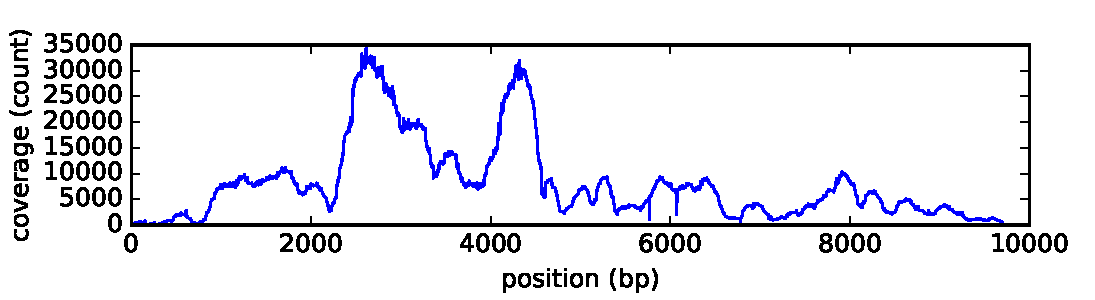
\includegraphics[width=0.99\linewidth]{coverage.pdf}
\caption{}
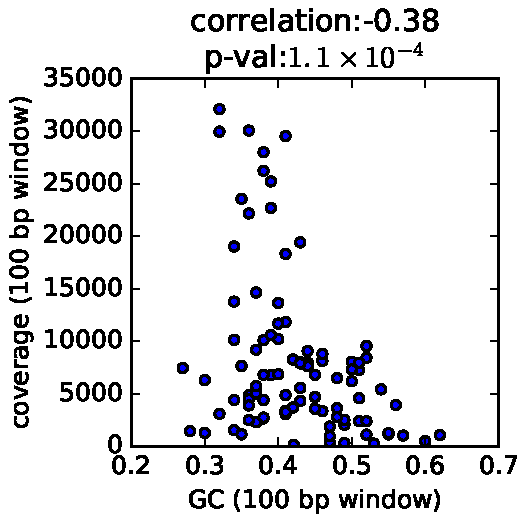
\includegraphics[width=0.4\linewidth]{correlation.pdf}
\caption{}
\end{subfigure}
\caption{a) Mapping coverage of mi-seq reads, excluding introns, taken from RNA $\rightarrow$ cDNA to the HIV genome (K03455.1). I filtered out reads with average quality scores less than 38. b) Over each 100 bp window, I averaged the read coverage and GC content, and compared the two. I found a negative correlation between GC content and read coverage. Further analysis will need to performed to determine if this negative correlation is caused by a particular gene or cluster of positions. }\label{fig:QC38}
\end{figure}

\graphicspath{{"./STAR_out/"}}
\begin{figure}
\begin{subfigure}{1\textwidth}
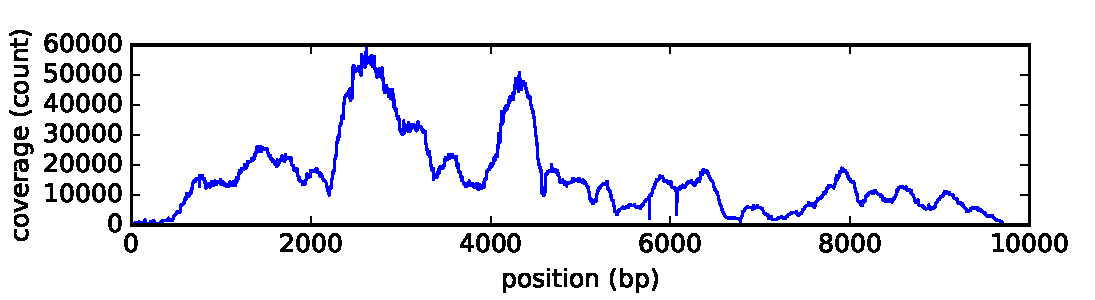
\includegraphics[width=0.99\linewidth]{pipeline_test_QC0coverage.pdf}
\caption{}
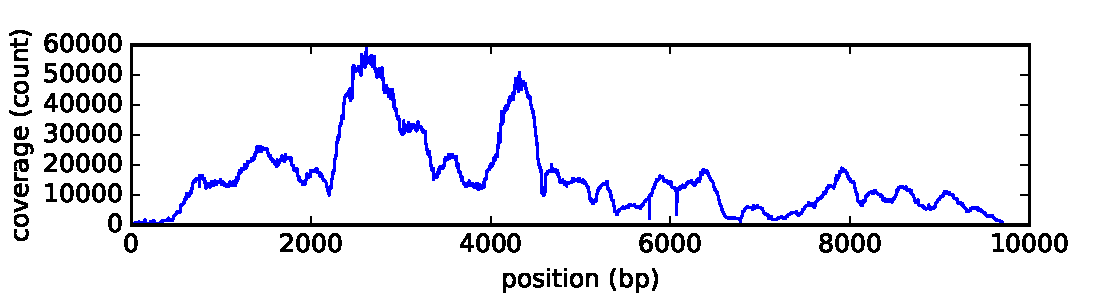
\includegraphics[width=0.99\linewidth]{pipeline_test_QC10coverage.pdf}
\caption{}
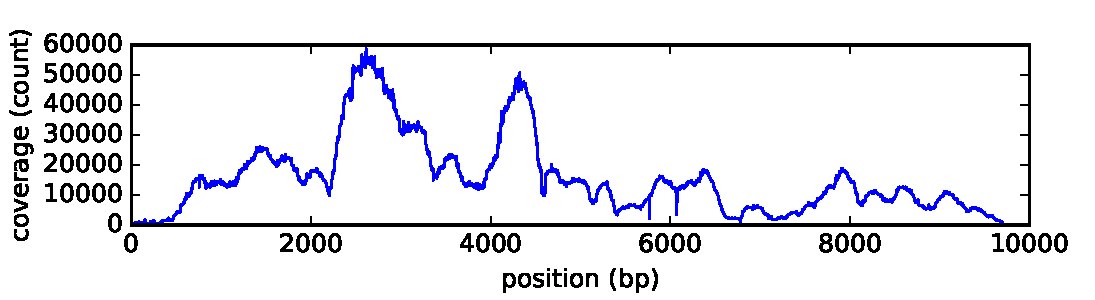
\includegraphics[width=0.99\linewidth]{pipeline_test_QC20coverage.pdf}
\caption{}
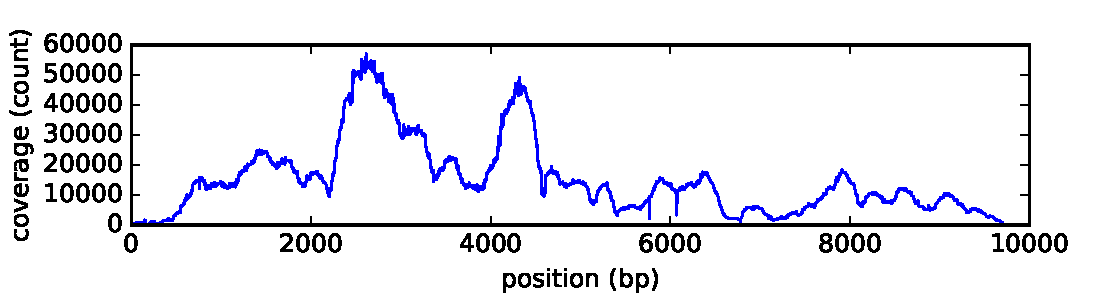
\includegraphics[width=0.99\linewidth]{pipeline_test_QC30coverage.pdf}
\caption{}
\end{subfigure}
\caption{ Mapping coverage of mi-seq reads, excluding introns, taken from RNA $\rightarrow$ cDNA to the HIV genome (K03455.1). I filtered out reads with average quality scores less than a) 0, b) 10, c) 20, and d)30. I found little difference between filterings, suggesting fairly consistent and high quality read maps. }\label{fig:coverage}
\end{figure}


\graphicspath{{"./STAR_out/"}}
\begin{figure}
\begin{subfigure}{0.4\textwidth}
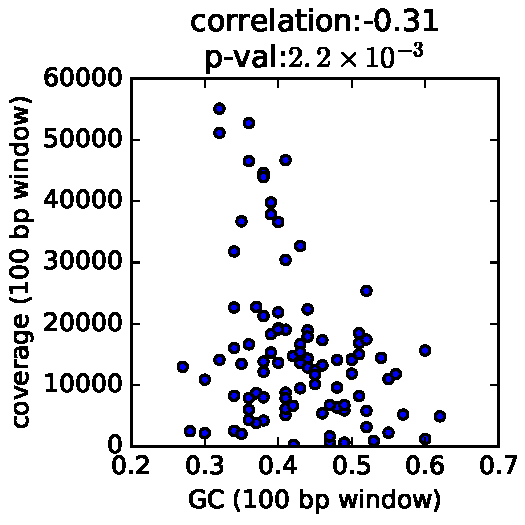
\includegraphics[width=0.99\linewidth]{pipeline_test_QC0correlation.pdf}
\caption{}
\end{subfigure}
\begin{subfigure}{0.4\textwidth}
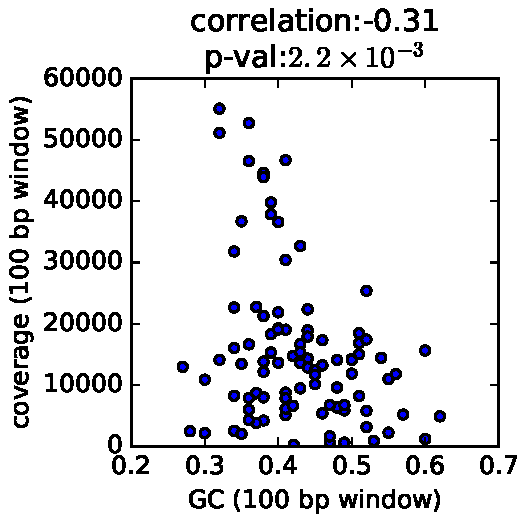
\includegraphics[width=0.99\linewidth]{pipeline_test_QC10correlation.pdf}
\caption{}
\end{subfigure}
\begin{subfigure}{0.4\textwidth}
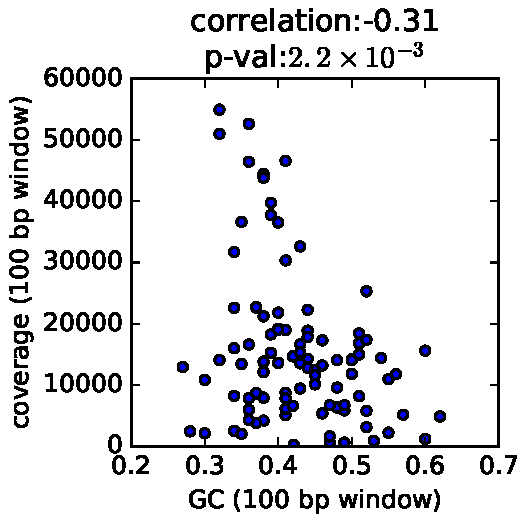
\includegraphics[width=0.99\linewidth]{pipeline_test_QC20correlation.pdf}
\caption{}
\end{subfigure}
\begin{subfigure}{0.4\textwidth}
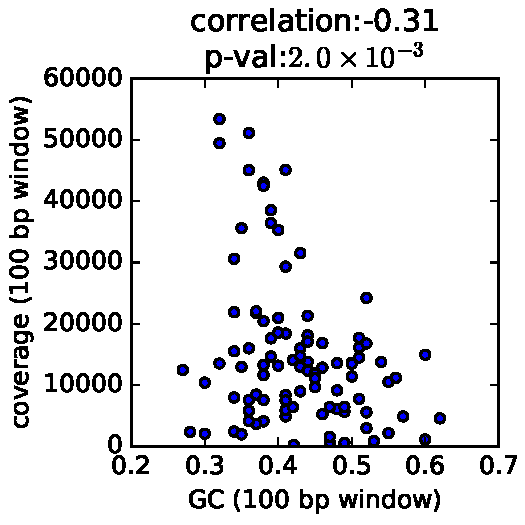
\includegraphics[width=0.99\linewidth]{pipeline_test_QC30correlation.pdf}
\caption{}
\end{subfigure}
\caption{ Comparing coverage by position (excluding introns) to GC content yielded fairly consistent correlations for reads filtered by average quality scores less than a) 0, b) 10, c) 20, and d)30. p-values only drop a small fraction for QC control cutoff of 30.}\label{fig:GC_content}
\end{figure}

%%% Bibliography
\bibliographystyle{apalike}
\bibliography{mapping_report}
%\clearpage

\end{document}